%--------------------------------------------------------------------------------------------------%
%	The MIT License (MIT)
%
%	Copyright (c) 2019 Jan Küster
%
%	Permission is hereby granted, free of charge, to any person obtaining a copy
%	of this software and associated documentation files (the "Software"), to deal
%	in the Software without restriction, including without limitation the rights
%	to use, copy, modify, merge, publish, distribute, sublicense, and/or sell
%	copies of the Software, and to permit persons to whom the Software is
%	furnished to do so, subject to the following conditions:
%	
%	THE SOFTWARE IS PROVIDED "AS IS", WITHOUT WARRANTY OF ANY KIND, EXPRESS OR
%	IMPLIED, INCLUDING BUT NOT LIMITED TO THE WARRANTIES OF MERCHANTABILITY,
%	FITNESS FOR A PARTICULAR PURPOSE AND NONINFRINGEMENT. IN NO EVENT SHALL THE
%	AUTHORS OR COPYRIGHT HOLDERS BE LIABLE FOR ANY CLAIM, DAMAGES OR OTHER
%	LIABILITY, WHETHER IN AN ACTION OF CONTRACT, TORT OR OTHERWISE, ARISING FROM,
%	OUT OF OR IN CONNECTION WITH THE SOFTWARE OR THE USE OR OTHER DEALINGS IN
%	THE SOFTWARE.
%	
%
%--------------------------------------------------------------------------------------------------%
\documentclass[11pt,A4]{article}	
\usepackage[utf8]{inputenc}		
\usepackage{xstring, xifthen}

\usepackage{CormorantGaramond}

\usepackage[T1]{fontenc}
\usepackage{moresize}
\usepackage{fontawesome}

\newcommand{\vcenteredinclude}[1]{\begingroup
	\setbox0=\hbox{\includegraphics{#1}}%
	\parbox{\wd0}{\box0}\endgroup}

\newcommand*{\vcenteredhbox}[1]{\begingroup
	\setbox0=\hbox{#1}\parbox{\wd0}{\box0}\endgroup}

\newcommand{\icon}[3] { 							
	\makebox(#2, #2){\textcolor{maincol}{\csname fa#1\endcsname}}
}	

\newcommand{\icontext}[4]{ 						
	\vcenteredhbox{\icon{#1}{#2}{#3}}  \hspace{2pt}  \parbox{0.9\mpwidth}{\textcolor{#4}{#3}}
}

\newcommand{\iconhref}[4]{ 						
	\vcenteredhbox{\icon{#1}{#2}{black}}  \hspace{2pt} \href{#4}{{#3}}
}

\newcommand{\iconemail}[5]{ 						
	\vcenteredhbox{\icon{#1}{#2}{#5}}  \hspace{2pt} \href{mailto:#4}{\textcolor{#5}{#3}}
}

%----------------------------------------------------------------------------------------
%	PAGE LAYOUT  DEFINITIONS
%----------------------------------------------------------------------------------------

% page outer frames (debug-only)
%\usepackage{showframe}		

% we use paracol to display breakable two columns
\usepackage{paracol}

\usepackage[a4paper]{geometry}
\geometry{top=1cm, bottom=1cm, left=1cm, right=1cm}

\usepackage{fancyhdr}
\pagestyle{empty}

% space between header and content
% \setlength{\headheight}{0pt}

% indentation is zero
\setlength{\parindent}{0mm}

\usepackage{array}
\newcolumntype{x}[1]{%
	>{\raggedleft\hspace{0pt}}p{#1}}%

\usepackage{graphicx}
% use this for floating figures
% \usepackage{wrapfig}
% \usepackage{float}
% \floatstyle{boxed} 
% \restylefloat{figure}

%for drawing graphics		
\usepackage{tikz}				
\usetikzlibrary{shapes, backgrounds, mindmap, trees}

\usepackage{transparent}
\usepackage{color}
% primary color
\definecolor{maincol}{RGB}{ 169, 10, 10 }
% accent color, secondary
 \definecolor{accentcol}{RGB}{ 250, 150, 10 }
% dark color
%\definecolor{darkcol}{RGB}{ 10, 100, 100 }
\definecolor{darkcol}{rgb}{0.23, 0.27, 0.29}
% light color
\definecolor{lightcol}{RGB}{245,245,245}

\usepackage[hidelinks]{hyperref}
\hypersetup{
	colorlinks=true,
	linkcolor=blue,
	filecolor=magenta,      
	urlcolor=darkcol,
}

% returns minipage width minus two times \fboxsep
% to keep padding included in width calculations
% can also be used for other boxes / environments
\newcommand{\mpwidth}{\linewidth-\fboxsep-\fboxsep}

%============================================================================%
%
%	CV COMMANDS
%
%============================================================================%

%----------------------------------------------------------------------------------------
%	 CV LIST
%----------------------------------------------------------------------------------------
\newcommand{\cvlist}[1] {
	\begin{itemize}{#1}\end{itemize}
}

%----------------------------------------------------------------------------------------
%	 CV TEXT
%----------------------------------------------------------------------------------------
\newcommand{\cvtext}[1] {
	\begin{tabular*}{1\mpwidth}{p{0.98\mpwidth}}
		\parbox{1\mpwidth}{#1}
	\end{tabular*}
}

%----------------------------------------------------------------------------------------
%	CV SECTION
%----------------------------------------------------------------------------------------
\newcommand{\cvsection}[1] {
	\vspace{14pt}
	\cvtext{
		\textbf{\LARGE{\textcolor{darkcol}{{#1}}}}\\[-4pt]
		\textcolor{maincol}{ \rule{0.1\textwidth}{2pt} } \\
	}
}

%----------------------------------------------------------------------------------------
%	META SKILL
%----------------------------------------------------------------------------------------
\newcommand{\cvskill}[3] {
	\begin{tabular*}{1\mpwidth}{p{0.72\mpwidth}  r}
		\textcolor{black}{\textbf{#1}} & \textcolor{maincol}{#2}\\
	\end{tabular*}%
	
	\hspace{4pt}
	\begin{tikzpicture}[scale=1,rounded corners=2pt,very thin]
	\fill [lightcol] (0,0) rectangle (1\mpwidth, 0.15);
	\fill [maincol] (0,0) rectangle (#3\mpwidth, 0.15);
	\end{tikzpicture}%
}


%----------------------------------------------------------------------------------------
%	 CV EVENT
%----------------------------------------------------------------------------------------
\newcommand{\cvevent}[4] {
	\parbox{\mpwidth}{
		\begin{tabular*}{1\mpwidth}{p{0.72\mpwidth}  r}
			\textcolor{black}{\textbf{#2}} & \colorbox{maincol}{\makebox[0.25\mpwidth]{\textcolor{white}{#1}}} \\
			\textcolor{maincol}{\textbf{#3}} & \\
		\end{tabular*}\\[8pt]
		
		\ifthenelse{\isempty{#4}}{}{
			\cvtext{#4}\\
		}
	}
	
	\vspace{14pt}
}

%----------------------------------------------------------------------------------------
%	 CV META EVENT
%----------------------------------------------------------------------------------------
\newcommand{\cvmetaevent}[4] {
	\textcolor{maincol} {\cvtext{\textbf{\begin{flushleft}#1\end{flushleft}}}}
	
	\ifthenelse{\isempty{#2}}{}{
		\textcolor{darkcol} {\cvtext{\textbf{#2}}\\[-12pt] }
	}
	
	\ifthenelse{\isempty{#3}}{}{
		\cvtext{{ \textcolor{darkcol} {#3} }}\\[-7.5pt]
	}
	
	\cvtext{#4}\\[10pt]
}
\usepackage{afterpage}
%----------------------------------------------------------------------------------------
%	 References
%----------------------------------------------------------------------------------------
\newcommand{\references}{
%	\newpage
%	\vspace*{2in}
	\afterpage{%
		\newgeometry{top=5cm, bottom=3cm, left=3cm, right=2cm}
		\cvsection{References}
		
		\cvtext{
			My advisor, professor Karri Muinonen\\
			Department of Physics\\
			University of Helsinki\\
			\href{mailto:karri.muinonen@helsinki.fi}{karri.muinonen@helsinki.fi}\\
			
			Frequent collaborator, professor Alex Lazarian\\
			Department of Astronomy\\
			University of Wisconsin/Madison\\
			\href{mailto:alazarian@facstaff.wisc.edu}{alazarian@facstaff.wisc.edu}\\
			
			Collaborator, Dr. Gorden Videen\\
			Army Research Laboratory\\
			Maryland, US\\
			\href{mailto:gorden.videen@gmail.com}{gorden.videen@gmail.com}
		}
		\restoregeometry
	} 
	
}

%----------------------------------------------------------------------------------------
%	 Cover letter
%----------------------------------------------------------------------------------------
\newcommand{\coverletter}{	
	\afterpage{%
		\newgeometry{top=3cm, bottom=3cm, left=2cm, right=2cm}
		\cvtext{
			\flushright
			\today\\[10pt]
			
			University of Helsinki\\
			Department of Physics\\
			Gustaf Hällströmin katu 2\\
			PL 64, Helsinki, Finland\\
			\href{mailto:joonas.herranen@helsinki.fi}{joonas.herranen@iki.fi}
			
			\flushleft 
	
			\cvtext{
				\Large{
					Post doc position (F*M), job ID: IWF035PD220\\[2pt]
				}
				\large{
					Space Research Institute (IWF)\\
					Austrian Academy of Sciences\\
				}
			
				Dear Dr. Mannel,\\
				
				I apply for the post doc position mentioned in the title. I defend my thesis, titled \emph{Dynamical response of small particles to light scattering}, on August 25th, 2020, with Dr. B-G Andersson as my opponent. \\
				
				My research, as my teaching, experience focusses on numerical light scattering methods, applied to cosmic dust and other small particles, including cometary dust and particles trapped in optical tweezers. The main computational tools I have used are Fortran (numerical light scattering) and Python (input data and particle shape generation, data analysis and visualization). I also have a solid understanding of the electromagnetic theory.\\
				
				I earned all my academic degrees in the University of Helsinki. During my time there, I have extensively studied theoretical physics, physics, mathematics, and chemistry. In addition I am a fully qualified teacher up to the secondary level in Finland. The extensive coverage of my knowledge is a strength and allows me to collaborate in many things, even if it means relative lack of depth of knowledge in fields other than my own expertise, scattering and dynamics of small particles.\\
				
				In the near future, I expect to pursue new research goals. New vantage points will hopefully strengthen my qualities as a scientist.\\
				
				After my graduation, I will append the application with my study certificates.\\
				
				\flushright
				Sincerely,\\[15pt]
				
\includegraphics[width=0.23\mpwidth]{sign}\\
				Joonas Herranen 
				
				\flushleft
			\textit{	Attachments:\\
				1) Study transcript from the University of Helsinki}
			}
		}
		\restoregeometry
	}
}

\usepackage{pdfpages}
\newcommand{\attachments}{
	\afterpage{
		\newgeometry{top=3cm, bottom=3cm, left=2cm, right=2cm}
		\cvsection{Attachment 1: Transcript}
		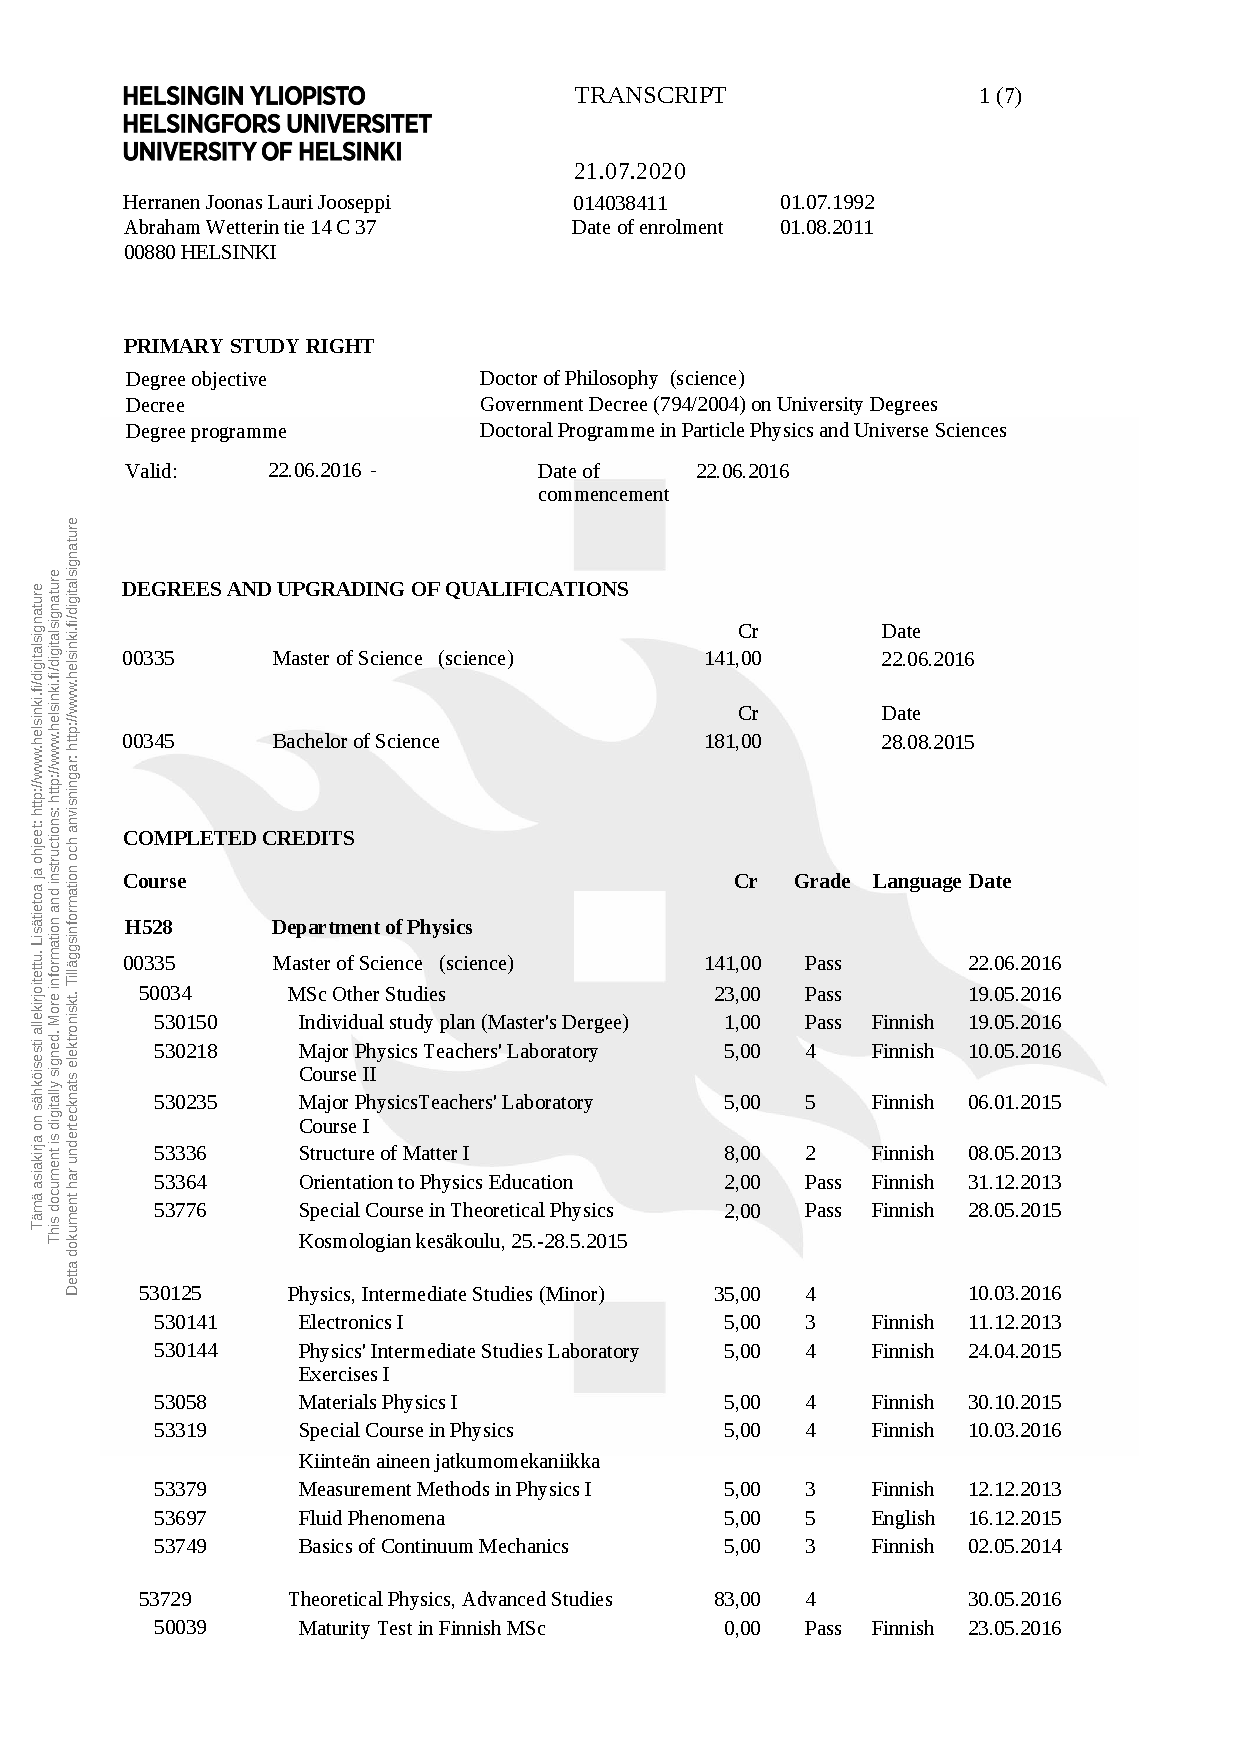
\includepdf[pages={1-7}]{transcript.pdf}
	}	
}


\begin{document}
	\columnratio{0.31}
	\setlength{\columnsep}{2.2em}
	\setlength{\columnseprule}{4pt}
	\colseprulecolor{lightcol}
	\begin{paracol}{2}
		\begin{leftcolumn}
			
			\cvsection{Personal information}
			
			\vspace*{-4pt}
			\icontext{Male}{12}{ 1 July 1992, Helsinki, Finland}{black}\\[3pt]
			\icontext{MapMarker}{12}{ Abraham Wetterin tie 14 C 37\\00880 Helsinki, Finland}{black}\\[3pt]
			\icontext{MobilePhone}{12}{ +358 45 356 2399}{black}\\[3pt]
			\iconemail{Envelope}{12}{ joonas.herranen@iki.fi}{joonas.herranen@iki.fi}{black}\\[3pt]
			\iconhref{Github}{12}{github.com/jherrane}{https://github.com/jherrane}\\[-15pt]
			
			\cvsection{Research profile}
			\\[-15pt]
			\cvmetaevent
			{Numerical light scattering}
			{}
			{}
			{ Development and application of a state-of-the-art efficient scattering solver for irregular scatterers, modelling especially the dynamical effects of radiation. }
			\\[-15pt]
			\cvmetaevent
			{Cosmic dust}
			{}
			{}
			{ Modelling shapes of dust grains and aggregates and their scattering properties is an integral part of e.g. understanding the radiative torque theory of dust and, further, the polarization of scattered and emitted light by dust.}
			\\[-15pt]
			\cvmetaevent
			{Optical tweezers}
			{}
			{}
			{ Full dynamical simulations allow modelling optical tweezers, where small particles can be suspended and manipulated by light.}\\[-20pt]
			
			\cvsection{Education}
			\\[-15pt]
			\cvmetaevent
			{2016 -- Aug 2020 (planned)}
			{PhD Astronomy}
			{University of Helsinki}
			{ Research under the supervision of prof. Karri Muinonen
			}\\[-20pt]
			\cvmetaevent
			{2015 -- 2016}
			{MSc Theoretical Physics}
			{University of Helsinki}
			{ \href{https://studies.helsinki.fi/instructions/article/grades-and-assessment}{Overall grade 4/5}
				
				My MSc thesis started my PhD research, and earned the highest grade of Laudatur.
			}
			\\[-20pt]
			\cvmetaevent
			{2012 -- 2015}
			{BSc Theoretical Physics}
			{}
			{University of Helsinki}
			\vfill\null
%			\newpage
			\cvsection{Other education}
			\\[-20pt]
			\cvmetaevent
			{2015 -- 2019}
			{Subject teacher}
			{University of Helsinki}
			{ Qualification for teaching Physics, Mathematics, Chemistry and IT up to the secondary level in Finland.
			}
			
			\cvsection{Skills}
			
			\cvskill{ Fortran, Python,
				Matlab} {5+ yrs} {1} \\[-2pt]
			
			\cvskill{ Linux, Git, \LaTeX} {4+ yrs} {0.95} \\[-2pt]
			
			\cvskill{ Html/CSS, SQL} {3+ yrs} {0.66} \\[-2pt]
			
			\cvsection{Language proficiency}
			
			\cvskill{Finnish}{Native}{} \\[-2pt]
			
			\cvskill{English}{Fluent}{0.9} \\[-2pt]
			
			\cvskill{Swedish}{\hspace{-38pt}Bureaucratese}{0.5} \\[-2pt]
			
			\cvskill{Japanese}{\hspace{-40pt}Conversational}{0.4} \\[-2pt]
			
			\cvsection{Additional activities}
			\vspace*{-20pt}
			\cvmetaevent
			{2020, Helsinki}
			{The Night of Science}
			{Bad Sci-Fi Night}
			{ \vspace*{-2pt}A popular science lecture on science fiction tropes and related physics.}
			
			\vspace*{-20pt}
			\cvmetaevent
			{2018, 2019, Helsinki Observatory}
			{International Asteroid Day}
			{}
			{\vspace*{4pt} Organizer at the Helsinki Observatory's exhibition for general public as a part of the international event.}
			\vfill\null
%			\mbox{} % hotfix to place qrcode on the bottom when there are not other elements
			
		\end{leftcolumn}
		\begin{rightcolumn}
			
			\fcolorbox{white}{darkcol}{\begin{minipage}[c][2.cm][c]{1\mpwidth}
					\begin {center}
					\huge{ \textbf{ \textcolor{white}{ {Joonas Herranen} } } } \\[4pt]
					\large{ \textcolor{white} {Curriculum Vitae} }
					\end {center}
			\end{minipage}} 
			
			\cvsection{Publications}
			
			\cvtext{
				
				Herranen, J. 2020, \emph{\href{https://doi.org/10.3847/1538-4357/ab8009}{Rotational disruption of nonspherical cometary dust particles by radiative torques}}, Astrophysical Journal, 893, 109. \\[-5pt]
				
				Herranen, J., Markkanen, J., Videen, G., \& Muinonen, K. 2019, \emph{\href{https://doi.org/10.1371/journal.pone.0225773}{Non-spherical particles in optical tweezers: a numerical solution}}, PLOS ONE, 12(14): e0225773.\\[-5pt]
				
				Herranen, J., Lazarian, A., \& Hoang, T. 2019, \emph{\href{https://doi.org/10.3847\%2F1538-4357\%2Fab1eb3}{Radiative torques of irregular grains: describing the alignment of a grain ensemble}}, Astrophysical Journal, 878, 96.\\[-5pt]
				
				Herranen, J., Markkanen, J., \& Muinonen, K. 2018, \emph{\href{https://doi.org/10.1016/j.jqsrt.2017.09.033}{Polarized scattering by Gaussian random particles under radiative torques}}, Journal of Quantitative Spectroscopy and Radiative Transfer, 205, 40.\\[-5pt]
				
				Herranen, J., Markkanen, J., \& Muinonen, K. 2017, \emph{\href{https://doi.org/10.1002/2017RS006333}{Dynamics of small particles in electromagnetic radiation fields: A numerical solution}}, Radio Science, 52, 1016.\\[-5pt]
				
				Herranen, J., Markkanen, J., \& Muinonen, K. (2016). \emph{\href{https://doi.org/10.1109/URSI-EMTS.2016.7571366}{Dynamics of Interstellar Dust Particles in Electromagnetic Radiation Fields}} in 2016 URSI International Symposium on Electromagnetic Theory (EMTS) (p. 251-254). New York: IEEE.
				
			}
			
			\cvsection{Other publications}
			
			\cvtext{
				
				Herranen, J., \& Lazarian, A. 2020, \emph{Alignment of irregular grains by radiative torques: efficiency study}, Astrophysical Journal, submitted.\\
				
				Herranen, J. 2020, \emph{Dynamical response of small particles to light scattering}, Doctoral dissertation, ISBN 978-951-51-6118-5 (pdf), ISSN 1799-3024, University of Helsinki Report Series in Astronomy, No. 24.
				
			}
			
			\cvsection{Grants and fellowships}
			
			\cvevent
			{2017 -- 2020}
			{UH funded salary position for a PhD candidate}
			{University of Helsinki}
			{}
			\vspace{-15pt}
			\cvevent
			{2015, 2013}
			{Study grant}
			{Student's foundation of Tavastia Nation}
			{}
			\vspace{-15pt}
			\cvevent
			{2015, 2013}
			{Undergraduate grant}
			{Fund for Mathematics and Natural Sciences}
			{}
			
			\vspace{-25pt}
			\cvsection{Awards and honors}
			
			\cvevent
			{2016}
			{Pro Gradu award exceptional MSc thesis}
			{Faculty of Science, University of Helsinki}
			{}
			\vspace{-15pt}
			\cvevent
			{2011}
			{Bronze medal in the International Chemistry Olympiad}
			{IChO 2011}
			{}
			
			\vfill\null
			\newpage
			\cvsection{Conferences}
			
			\cvevent
			{2020}
			{EPSC}
			{Virtual conference}
			{}
			\vspace*{-15pt}
			\cvevent
			{2019}
			{EPSC / DPS}
			{Geneva, Switzerland}
			{}
			\vspace*{-15pt}
			\cvevent
			{2018, 2019}
			{Cosmic Dust}
			{Sagamihara, Japan; Narashino, Japan}
			{}
			\vspace*{-15pt}
			\cvevent
			{2018}
			{ELS XVII / Laser-Light and Interactions with Particles (LIP) 2018}
			{College Station, TX}
			{}
			\vspace*{-15pt}
			\cvevent
			{2017}
			{EPSC}
			{Riga, Latvia}
			{}
			\vspace*{-15pt}
			\cvevent
			{2017}
			{Electromagnetic and Light Scattering (ELS) XVI}
			{College Park, MD}
			{}
			\vspace*{-15pt}
			\cvevent
			{2017}
			{Bremen Workshop on Light Scattering}
			{Bremen, Germany}
			{}
			\vspace*{-15pt}
			\cvevent
			{2016}
			{Annual Meeting for Division for Planetary Sciences (DPS) / European Planetary Science Conference (EPSC)}
			{Pasadena, CA}
			{}
			\vspace*{-15pt}
			\cvevent
			{2016}
			{Electromagnetic Theory Symposium (EMTS)}
			{Espoo, Finland}
			{}
			\vspace*{-15pt}
			
			\vspace*{-10pt}
			\cvsection{Teaching experience}
			
			\cvevent
			{2020}
			{Statistical Inversion Methods}
			{Assistant teacher}
			{}
			\vspace*{-15pt}
			\cvevent
			{2020}
			{Solar System Physics}
			{Assistant teacher}
			{}
			\vspace*{-15pt}
			\cvevent
			{2018, 2019}
			{Fundamentals of Astronomy I}
			{Assistant teacher}
			{}
			\vspace*{-15pt}
			\cvevent
			{2018}
			{Fundamentals of Astronomy II}
			{Assistant teacher}
			{}
			\vspace*{-15pt}
			\cvevent
			{2016, 2018}
			{Electromagnetic Scattering I}
			{Assistant teacher}
			{}
			\vspace*{-15pt}
			
			\vspace*{-10pt}
			\cvsection{Research experience}
			
			\cvevent
			{2019}
			{Visiting researcher}
			{University of Wisconsin/Madison}
			{\vspace*{-15pt}Two-month research visit to prof. A. Lazarian, focussed on improving the predictivity of radiative torque theory.}
			\vspace*{-15pt}
			\cvevent
			{2016 -- 2020}
			{Doctoral student}
			{University of Helsinki}
			{}
			% hotfixes to create fake-space to ensure the whole height is used
			%\mbox{}
			%\vfill
			%\mbox{}
			%\vfill
			%\mbox{}
			%\vfill
			%\mbox{}
		\end{rightcolumn}
	\end{paracol}
	
	\references
	\coverletter
	\attachments
	
\end{document}

